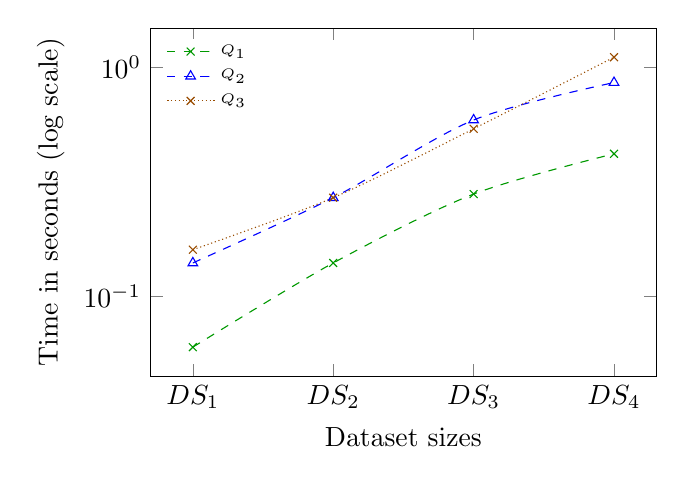
\begin{tikzpicture}
  \begin{loglogaxis}[xlabel={Dataset sizes},ylabel={Time in seconds (log scale)},%
    scaled x ticks = false, x tick label style = {/pgf/number format/fixed},scaled y ticks = false,%
    y tick label style = {/pgf/number format/fixed},enlargelimits=true,xtick={1,2,4,8},%
    xticklabels={$DS_{1}$,$DS_{2}$,$DS_{3}$,$DS_{4}$},log basis x=10,log basis y=10,unbounded coords=jump,xminorticks=false,%
    yminorticks=false,height=6cm,width=8cm,filter discard warning=false,%
    legend style={inner sep=0,legend columns=1,draw=none,font=\tiny,at={(0,0)},anchor=south east,legend pos=north west,anchor=north west,legend cell align=left}]

\addplot[smooth,dashed, color=green!60!black, every mark/.append style={solid},mark=x,] coordinates {
(1, 0.06)
(2, 0.14)
(4, 0.28)
(8, 0.42)
};
\addlegendentry{$Q_{1}$}
\addplot[smooth,dashed, color=blue, every mark/.append style={solid},mark=triangle,] coordinates {
(1, 0.14)
(2, 0.27)
(4, 0.59)
(8, 0.86)
};
\addlegendentry{$Q_{2}$}
\addplot[smooth,densely dotted, color=orange!60!black, every mark/.append style={solid},mark=x,] coordinates {
(1, 0.16)
(2, 0.27)
(4, 0.54)
(8, 1.11)
};
\addlegendentry{$Q_{3}$}
\end{loglogaxis}
\end{tikzpicture}


%%% Local Variables:
%%% mode: latex
%%% mode: flyspell
%%% mode: reftex
%%% TeX-master: "../../thesis"
%%% End:
